\documentclass[tikz]{standalone}
\usepackage{pgfplots}
\usepackage{xcolor} % For using hex colors
\usetikzlibrary{calc}
\definecolor{mycolor}{HTML}{ffd966} % Define custom color #ffd966
\definecolor{startcolor}{HTML}{ff6b6b} % Red color for start point
\definecolor{endcolor}{HTML}{4ecdc4} % Teal color for end point
\definecolor{arrowcolor}{HTML}{45b7d1} % Blue color for gradient descent arrow
\pgfplotsset{compat=1.18}

\begin{document}
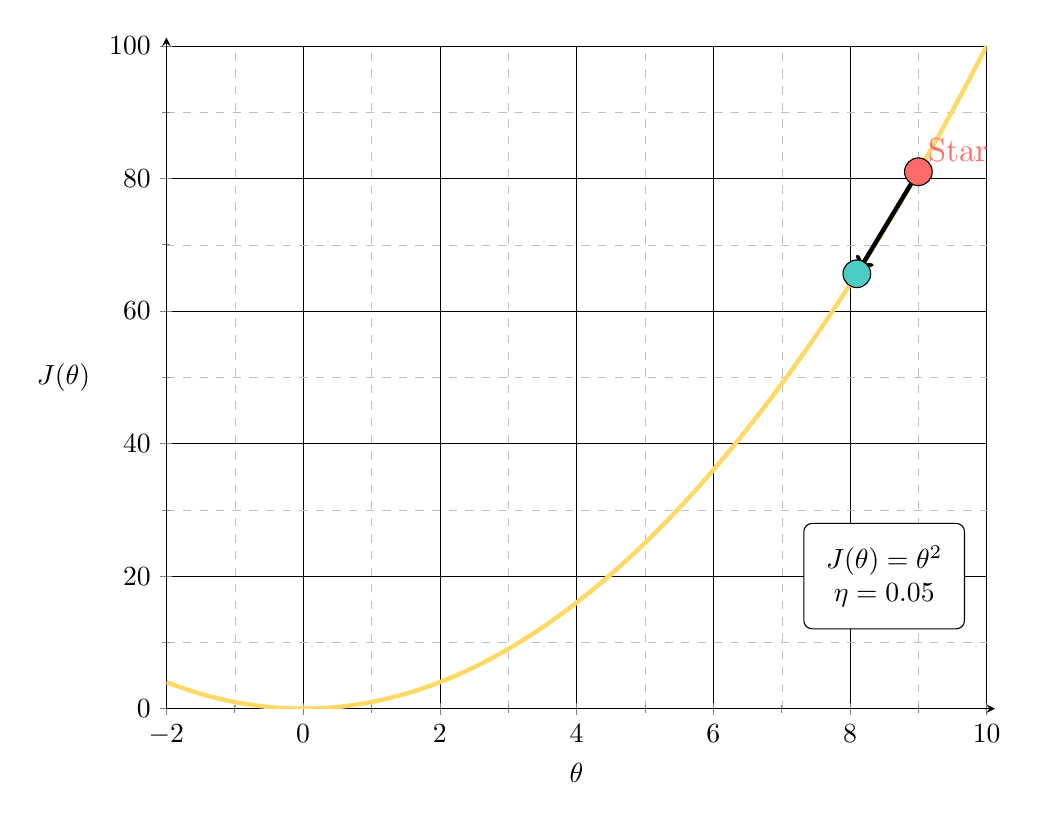
\begin{tikzpicture}
  \begin{axis}[
    % Draw only the bottom and left axes with arrow tips:
    axis lines=left,
    x axis line style={->,>=stealth, shorten >=-3pt},
    y axis line style={->,>=stealth, shorten >=-3pt},
    xlabel={\(\theta\)},
    ylabel={\(J(\theta)\)},
    % Rotate the y label so that it appears upside down:
    ylabel style={rotate=-90},
    xmin=-2, xmax=10,
    ymin=0, ymax=100,
    % Major ticks at integer values...
    xtick={-2,0,2,...,10},
    ytick={0,20,...,100},
    % One minor tick between each major tick:
    minor x tick num=1,
    minor y tick num=1,
    grid=both,
    % Grid styling:
    major grid style={line width=0.2pt,draw=black},
    minor grid style={line width=0.1pt,draw=gray!50,dashed},
    width=12cm,
    height=10cm,
  ]
    % Plot the function J(θ) = θ^2 over θ from 0 to 10 with a thicker line and custom color:
    \addplot[domain=-2:10, samples=200, ultra thick, color=mycolor] {x^2};
    
    % Starting point at x=9, J(9) = 81
    \addplot[only marks, mark=*, mark options={scale=2.5, fill=startcolor}] coordinates {(9,81)};
    
    % Calculate gradient descent step
    % At x=9, gradient = dJ/dx = 2x = 18
    % New x = x - learning_rate * gradient = 9 - 0.05 * 18 = 9 - 0.9 = 8.1
    % New J = (8.1)^2 = 65.61
    
    % End point after gradient descent
    \addplot[only marks, mark=*, mark options={scale=2.5, fill=endcolor}] coordinates {(8.1,65.61)};
    
    % Draw arrow from start to end point
    \addplot[->, ultra thick, color=black, shorten >=2pt, shorten <=2pt] coordinates {(9,81) (8.1,65.61)};
    
    % Add labels for the points
    \node[above right, color=startcolor, font=\large] at (axis cs:9,81) {Start: $\theta=9$};
    
    % Add legend box with function notation and learning rate
    \node[draw=black, fill=white, rounded corners=3pt, inner sep=8pt, font=\normalsize, align=center] at (axis cs:8.5,20) {
      $J(\theta) = \theta^2$ \\
      $\eta = 0.05$
    };
    
  \end{axis}
\end{tikzpicture}
\end{document}
